\documentclass[12pt]{article}
\usepackage[utf8]{inputenc}
\usepackage[T1]{fontenc}
\usepackage[spanish,es-tabla,es-noindentfirst]{babel}
\decimalpoint
\usepackage{amsmath,amssymb}
\usepackage[margin=2.5cm]{geometry}
\usepackage{booktabs}
\usepackage{caption}
\usepackage{graphicx}
\usepackage{float}
\usepackage{placeins}
\usepackage{enumitem}
\usepackage[colorlinks=true,linkcolor=black,urlcolor=blue]{hyperref}
\usepackage{setspace}
\onehalfspacing
\setlength{\parskip}{4pt}

\begin{document}

\begin{center}
{\large \textbf{UNIVERSIDAD DEL DESARROLLO}}\\
{\large \textbf{FACULTAD DE ECONOMÍA Y NEGOCIOS}}\\
{\large \textbf{PhD in Business Economics}}

\vspace{1em}

{\Large \textbf{MÉTODOS CUANTITATIVOS DE INVESTIGACIÓN EN NEGOCIOS}}

\vspace{0.7em}

{\large \textbf{TAREA \#2--3--4: RESPUESTAS}}
\end{center}

\vspace{1em}

\textbf{Fecha de entrega:} 17 de julio de 2026

\textbf{Ponderación:} 65\%

\textbf{Estudiante:} J. Sebastián Becerra C.

\vspace{1em}

\section*{Enunciado general}

Para cada una de las preguntas, se describen claramente los pasos seguidos y se adjuntan los resultados de los análisis efectuados durante el proceso. Los cálculos fueron realizados en Python y se encuentran respaldados por notebooks individuales reproducibles, uno por pregunta, incluidos en la carpeta de entrega.

\subsection*{Notebooks reproducibles en Google Colab}

Los análisis de cada pregunta pueden revisarse y ejecutarse en Google Colab desde los siguientes vínculos:
\begin{itemize}\itemsep2pt
\item \href{https://colab.research.google.com/github/sebabecerra/Metodos-Cuantitativos-DEN/blob/main/Tarea2/notebooks/Tarea_2_P1_Mediacion_Moderada.ipynb}{Pregunta 1: mediación moderada}.
\item \href{https://colab.research.google.com/github/sebabecerra/Metodos-Cuantitativos-DEN/blob/main/Tarea2/notebooks/Tarea_2_P2_Analisis_Factorial.ipynb}{Pregunta 2: análisis factorial exploratorio}.
\item \href{https://colab.research.google.com/github/sebabecerra/Metodos-Cuantitativos-DEN/blob/main/Tarea2/notebooks/Tarea_2_P3_SEM.ipynb}{Pregunta 3: CFA, SEM y comparación por género}.
\item \href{https://colab.research.google.com/github/sebabecerra/Metodos-Cuantitativos-DEN/blob/main/Tarea2/notebooks/Tarea_2_P4_MANOVA.ipynb}{Pregunta 4: MANOVA factorial}.
\end{itemize}

\newpage

\section*{Pregunta 1}


\subsection*{Enunciado}

Para cada una de las preguntas, describa claramente los pasos seguidos y adjunte los resultados de los análisis efectuados durante el proceso.

Como parte de una investigación en la que está participando, se le ha solicitado realizar un análisis de un modelo que explica la relación entre la presión competitiva del mercado y el desempeño innovador de la empresa. En este modelo (ver figura 1) se plantea que el efecto de la presión competitiva sobre el desempeño innovador está mediado por la conducta innovadora de los empleados, pero que esta relación depende de la cultura de tolerancia al fracaso de la organización.

\begin{figure}[H]
\centering
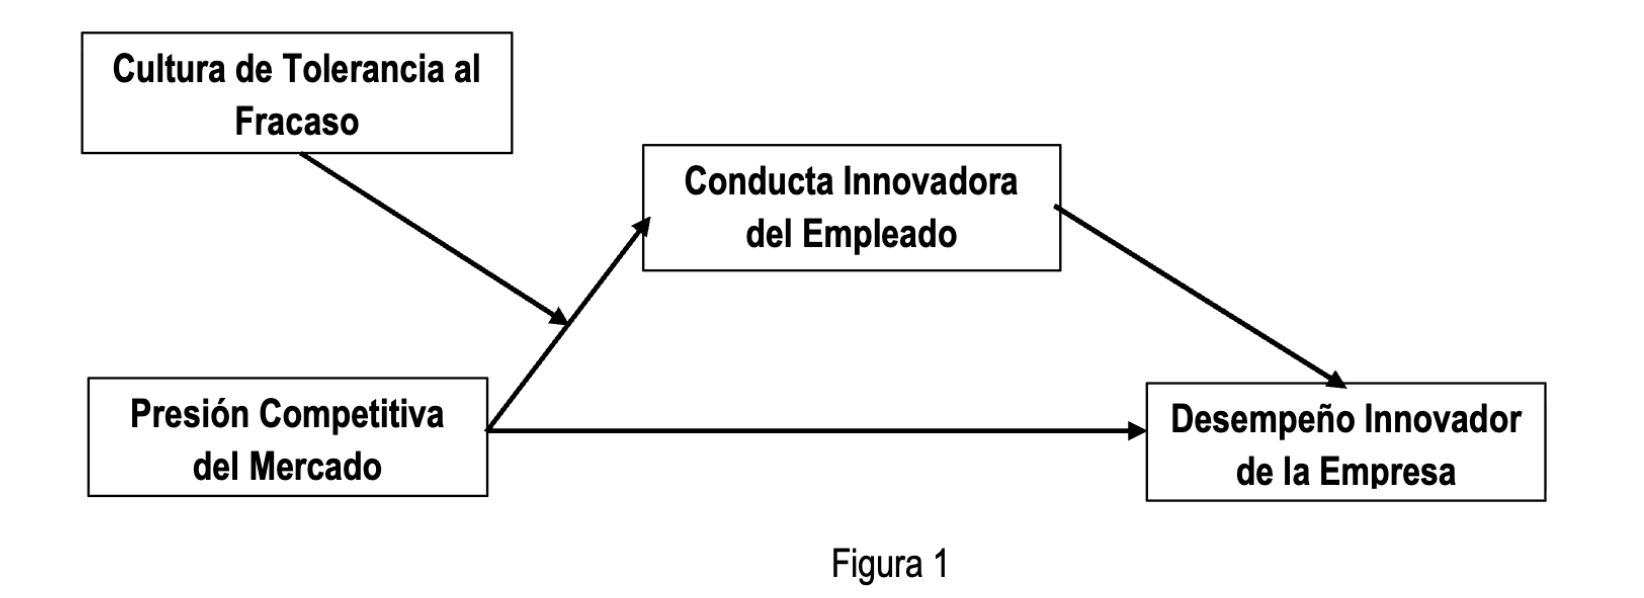
\includegraphics[width=0.92\textwidth]{assets/figura_1_modelo.png}
\caption{Figura 1}
\end{figure}

Las variables del modelo se explican a continuación:
\begin{itemize}\itemsep2pt
\item \textbf{Presión Competitiva del Mercado:} Nivel de rivalidad y cambios tecnológicos en el sector, medida en una escala de 1 a 10, donde un mayor número representa una mayor presión competitiva.
\item \textbf{Cultura de Tolerancia al Fracaso:} Grado en que la gerencia castiga o premia los errores al experimentar, medida en una escala de 1 a 7, donde un mayor número representa una mayor tolerancia al fracaso por parte de la gerencia.
\item \textbf{Conducta Innovadora del Empleado:} Generación e implementación de ideas nuevas en el trabajo, medida como el número de ideas propuestas por el empleado en los últimos 5 años.
\item \textbf{Desempeño Innovador de la Empresa:} Generación exitosa de nuevos productos o servicios para el mercado, medida como el porcentaje de ingresos de la organización proveniente de productos o servicios lanzados los últimos 5 años.
\end{itemize}

Con los datos de las respuestas 200 empleados de 200 empresas distintas (contenidos en la base \textit{Med\_Mod.sav}), usted deberá:
\begin{enumerate}[label=\alph*)]\itemsep2pt
\item Plantear el modelo en forma de hipótesis.
\item Evaluar cada una de estas hipótesis.
\item Interpretar los resultados.
\end{enumerate}

\subsection*{Respuesta}

\subsection*{Justificación conceptual del modelo}

El objetivo de este análisis es comprender de qué manera la presión competitiva del mercado puede traducirse en un mayor desempeño innovador de la empresa. El planteamiento no supone que esta relación ocurra de forma exclusivamente directa. Por el contrario, propone que la presión competitiva primero modifica el comportamiento de los empleados, incentivándolos a generar, promover e implementar nuevas ideas. Estas conductas innovadoras constituirían el mecanismo mediante el cual una condición externa del mercado termina produciendo resultados innovadores a nivel organizacional.

Desde esta perspectiva, la conducta innovadora del empleado funciona como una variable mediadora. Su papel consiste en explicar cómo la presión competitiva se transforma en desempeño innovador. La mediación, por tanto, no se limita a comprobar si dos variables están relacionadas, sino que busca identificar el proceso intermedio que conecta ambas.

Sin embargo, el modelo también reconoce que la presión competitiva no necesariamente genera la misma respuesta en todas las organizaciones. En una empresa donde los errores derivados de la experimentación son castigados, los trabajadores podrían reaccionar a la presión evitando riesgos o reduciendo su disposición a proponer nuevas ideas. En cambio, cuando la organización acepta que el fracaso forma parte del proceso de aprendizaje, la misma presión competitiva podría convertirse con mayor facilidad en una fuente de experimentación e innovación.

Por esta razón, la cultura de tolerancia al fracaso actúa como variable moderadora. Su función es modificar la intensidad de la relación entre presión competitiva y conducta innovadora. Al combinarse el mecanismo de mediación con esta condición de moderación, el modelo corresponde a una mediación moderada de primera etapa. En esta tarea no se ejecuta la macro PROCESS; el modelo se estima directamente mediante regresiones OLS equivalentes al sistema estadístico requerido.

\subsection*{Especificación formal del modelo}

Las variables del modelo se organizan de la siguiente manera:

\begin{table}[H]
\centering
\caption{Variables consideradas en el modelo}
\begin{tabular}{lll}
\toprule
Rol en el modelo & Variable & Símbolo \\
\midrule
Variable independiente & Presión competitiva del mercado & $X$ \\
Variable mediadora & Conducta innovadora del empleado & $M$ \\
Variable moderadora & Cultura de tolerancia al fracaso & $W$ \\
Variable dependiente & Desempeño innovador de la empresa & $Y$ \\
\bottomrule
\end{tabular}
\end{table}

El modelo se estima mediante tres regresiones relacionadas entre sí. Cada una responde una pregunta distinta y permite evaluar una parte específica del mecanismo propuesto.

\subsubsection*{Primera regresión: explicación de la conducta innovadora}

La primera ecuación toma la conducta innovadora como variable dependiente. Su propósito es determinar si la presión competitiva aumenta la conducta innovadora de los empleados y, al mismo tiempo, si esa relación cambia según el nivel de tolerancia al fracaso.

\[
M=i_M+a_1X+a_2W+a_3(XW)+e_M
\]

En esta ecuación, $a_1$ representa el efecto de la presión competitiva cuando la tolerancia al fracaso se encuentra en su valor de referencia. El coeficiente $a_2$ representa el efecto de la tolerancia al fracaso cuando la presión competitiva se encuentra en su nivel de referencia. El término más importante para evaluar la moderación es $a_3$, porque indica si la pendiente entre presión competitiva y conducta innovadora cambia cuando aumenta la tolerancia al fracaso.

Si $a_3$ es positivo y significativo, se concluiría que la presión competitiva genera una mayor respuesta innovadora en organizaciones que aceptan con mayor facilidad los errores derivados de la experimentación.

\subsubsection*{Segunda regresión: explicación del desempeño innovador}

La segunda ecuación toma el desempeño innovador como variable dependiente. Su objetivo es determinar si la conducta innovadora de los empleados se traduce efectivamente en resultados innovadores para la empresa y si, una vez incorporado este mecanismo, persiste un efecto directo de la presión competitiva.

\[
Y=i_Y+c'X+bM+e_Y
\]

El coeficiente $b$ representa el efecto de la conducta innovadora sobre el desempeño innovador, manteniendo constante la presión competitiva. Por su parte, $c'$ representa el efecto directo residual de la presión competitiva sobre el desempeño, una vez que se incorpora al mediador.

Esta distinción es importante porque permite separar aquello que ocurre directamente desde la presión competitiva hacia el desempeño de aquello que ocurre indirectamente a través del comportamiento innovador de los empleados.

\subsubsection*{Tercera regresión: estimación del efecto total}

La tercera ecuación evalúa la relación global entre presión competitiva y desempeño innovador antes de introducir el mediador.

\[
Y=i_T+cX+e_T
\]

El coeficiente $c$ representa el efecto total de la presión competitiva sobre el desempeño innovador. Esta regresión permite establecer si existe una asociación global entre ambas variables, aunque por sí sola no permite identificar el mecanismo que genera dicha relación.

\subsubsection*{Efecto indirecto condicional}

A partir de las dos primeras ecuaciones se obtiene el efecto indirecto condicional:

\[
IE(W)=\left(a_1+a_3W\right)b
\]

Esta expresión muestra que el efecto indirecto de la presión competitiva sobre el desempeño innovador no es constante. Su magnitud depende del nivel de tolerancia al fracaso. Cuando $W$ aumenta, también cambia el efecto de $X$ sobre $M$ y, en consecuencia, cambia el efecto indirecto completo sobre $Y$.

\subsection*{Hipótesis}

A partir de esta especificación se plantean las siguientes hipótesis:

\begin{itemize}
    \item H1: La presión competitiva tiene un efecto total positivo sobre el desempeño innovador, de modo que $c>0$.
    
    \item H2: La presión competitiva incrementa la conducta innovadora del empleado, de modo que $a_1>0$.
    
    \item H3: La conducta innovadora incrementa el desempeño innovador de la empresa, de modo que $b>0$.
    
    \item H4: La conducta innovadora media significativamente la relación entre presión competitiva y desempeño innovador, por lo que $IE(W)\neq 0$.
    
    \item H5: La tolerancia al fracaso fortalece la relación entre presión competitiva y conducta innovadora, de modo que $a_3>0$.
    
    \item H6: El efecto indirecto de la presión competitiva sobre el desempeño innovador aumenta cuando la tolerancia al fracaso es mayor, por lo que el índice de mediación moderada $a_3b$ es positivo y distinto de cero.
\end{itemize}

\subsection*{Procedimiento de estimación}

El análisis se realizó utilizando las 200 observaciones disponibles en la base de datos, sin pérdidas de información en las variables incluidas en el modelo.

Antes de estimar las regresiones, la presión competitiva y la tolerancia al fracaso fueron centradas respecto de sus medias:

\[
X_c=X-\bar X
\]

\[
W_c=W-\bar W
\]

A continuación se construyó el término de interacción:

\[
X_cW_c=(X-\bar X)(W-\bar W)
\]

El centrado no cambia la significancia de la interacción ni el ajuste general del modelo. Su principal utilidad es facilitar la interpretación de los efectos principales. Después del centrado, el coeficiente de presión competitiva se interpreta en el nivel medio de tolerancia al fracaso, mientras que el coeficiente de tolerancia se interpreta en el nivel medio de presión competitiva.

Las tres ecuaciones fueron estimadas mediante mínimos cuadrados ordinarios. Para fortalecer la inferencia frente a posibles desviaciones de homocedasticidad, se utilizaron errores estándar robustos HC3.

Los efectos indirectos condicionales fueron evaluados mediante 5.000 remuestras bootstrap. Este procedimiento es especialmente apropiado para la mediación porque el producto de coeficientes no necesariamente sigue una distribución normal. En consecuencia, la significancia del efecto indirecto se determina observando si su intervalo de confianza bootstrap incluye o no el valor cero.

\subsection*{Resultados}

\subsubsection*{Primera regresión: conducta innovadora como variable dependiente}

La primera regresión evalúa simultáneamente el efecto de la presión competitiva, el efecto de la tolerancia al fracaso y la interacción entre ambas variables sobre la conducta innovadora.

\begin{table}[H]
\centering
\caption{Regresión del modelo del mediador}
\begin{tabular}{lcccc}
\toprule
Predictor & B & EE robusto & t & p \\
\midrule
Constante & 9.5207 & 0.0344 & 277.01 & $<0.001$ \\
Presión competitiva centrada ($a_1$) & 2.0008 & 0.0394 & 50.82 & $<0.001$ \\
Tolerancia al fracaso centrada ($a_2$) & 2.8732 & 0.0470 & 61.14 & $<0.001$ \\
Interacción $X_cW_c$ ($a_3$) & 0.5248 & 0.0389 & 13.48 & $<0.001$ \\
\bottomrule
\end{tabular}
\end{table}

El modelo explica el 98.05\% de la variación observada en la conducta innovadora, con un $R^2=0.9805$. Este nivel de ajuste indica que, dentro de la muestra analizada, la presión competitiva, la tolerancia al fracaso y su interacción explican una proporción muy elevada de las diferencias en conducta innovadora.

El coeficiente de presión competitiva es positivo y estadísticamente significativo. Dado que las variables fueron centradas, $a_1=2.0008$ representa el efecto de la presión competitiva cuando la tolerancia al fracaso se encuentra en su nivel promedio. En ese punto, un aumento de una unidad en presión competitiva se asocia con aproximadamente dos unidades adicionales de conducta innovadora.

La tolerancia al fracaso también presenta un efecto positivo y significativo. El coeficiente $a_2=2.8732$ indica que, cuando la presión competitiva se encuentra en su nivel promedio, una unidad adicional de tolerancia al fracaso se asocia con aproximadamente 2.87 unidades adicionales de conducta innovadora.

El resultado central de esta regresión corresponde al término de interacción. El coeficiente $a_3=0.5248$ es positivo y significativo, lo que demuestra que la relación entre presión competitiva y conducta innovadora no es constante. Por cada unidad adicional de tolerancia al fracaso, la pendiente de la presión competitiva aumenta en aproximadamente 0.525 unidades.

En términos sustantivos, la presión competitiva produce una respuesta innovadora más intensa cuando los empleados perciben que la organización acepta los errores propios de la experimentación. Por tanto, los resultados apoyan H2 y H5.

\subsubsection*{Segunda regresión: desempeño innovador como variable dependiente}

La segunda regresión evalúa si la conducta innovadora se transforma en desempeño innovador y si la presión competitiva conserva un efecto directo una vez incluido el mediador.

\begin{table}[H]
\centering
\caption{Regresión del modelo del resultado}
\begin{tabular}{lcccc}
\toprule
Predictor & B & EE robusto & t & p \\
\midrule
Constante & 1.4086 & 0.1564 & 9.01 & $<0.001$ \\
Presión competitiva centrada ($c'$) & 0.0265 & 0.0492 & 0.54 & 0.590 \\
Conducta innovadora ($b$) & 0.8577 & 0.0167 & 51.27 & $<0.001$ \\
\bottomrule
\end{tabular}
\end{table}

El modelo explica el 97.32\% de la variación del desempeño innovador, con un $R^2=0.9732$.

La conducta innovadora presenta un efecto positivo y altamente significativo sobre el desempeño innovador. El coeficiente $b=0.8577$ indica que, manteniendo constante la presión competitiva, una unidad adicional de conducta innovadora se asocia con un aumento aproximado de 0.858 unidades en el desempeño innovador.

Este resultado confirma que la conducta innovadora no constituye solamente una reacción de los empleados frente a la presión competitiva, sino que también se transforma en un resultado relevante para la empresa. Por tanto, se encuentra evidencia a favor de H3.

En cambio, el efecto directo residual de la presión competitiva no es significativo. El coeficiente $c'=0.0265$, con $p=0.590$, indica que, una vez incorporada la conducta innovadora, la presión competitiva no explica una variación adicional estadísticamente distinguible de cero en el desempeño innovador.

Este resultado sugiere que la asociación entre presión competitiva y desempeño innovador se transmite principalmente mediante la conducta innovadora. No obstante, la ausencia de significancia de $c'$ no constituye por sí sola una prueba suficiente de mediación. La evidencia formal debe obtenerse a partir de los intervalos bootstrap del efecto indirecto.

\subsubsection*{Tercera regresión: efecto total}

La regresión del efecto total muestra que la presión competitiva se relaciona positiva y significativamente con el desempeño innovador antes de incluir la conducta innovadora como mediador.

\[
c=2.0281,\qquad p<0.001
\]

Este coeficiente indica que una unidad adicional de presión competitiva se asocia, en promedio, con un aumento de 2.028 unidades en el desempeño innovador.

Como el efecto total es positivo y significativo, se encuentra evidencia a favor de H1. Sin embargo, esta regresión no permite determinar por qué ocurre la relación. Para comprender el mecanismo es necesario examinar conjuntamente las dos regresiones anteriores y los efectos indirectos condicionales.

\subsubsection*{Efectos indirectos condicionales}

El efecto indirecto se estimó en tres niveles representativos de tolerancia al fracaso: una desviación estándar bajo la media, la media y una desviación estándar sobre la media.

\begin{table}[H]
\centering
\caption{Efectos indirectos condicionales}
\begin{tabular}{@{}lcccc@{}}
\toprule
Nivel & Efecto $X\rightarrow M$ & Efecto indirecto & IC95\% inf. & IC95\% sup. \\
\midrule
Baja ($-1$ DE) & 1.6029 & 1.3748 & 1.2880 & 1.4620 \\
Medio & 2.0008 & 1.7162 & 1.6227 & 1.8104 \\
Alta ($+1$ DE) & 2.3988 & 2.0576 & 1.9319 & 2.1853 \\
\bottomrule
\end{tabular}
\end{table}

En los tres niveles de tolerancia al fracaso, los intervalos de confianza bootstrap excluyen el valor cero. Esto indica que la presión competitiva presenta un efecto indirecto significativo sobre el desempeño innovador a través de la conducta innovadora. Por tanto, se apoya H4.

Además, la magnitud del efecto indirecto aumenta sistemáticamente con la tolerancia al fracaso. Cuando la tolerancia es baja, el efecto indirecto es 1.3748. En el nivel medio aumenta a 1.7162 y, cuando la tolerancia es alta, alcanza 2.0576.

Este patrón muestra que la conducta innovadora transmite con mayor fuerza el efecto de la presión competitiva en organizaciones que presentan una cultura más tolerante frente al fracaso.

La existencia de mediación moderada se evalúa formalmente mediante el índice:

\[
a_3b=(0.5248)(0.8577)=0.4502
\]

El intervalo bootstrap al 95\% fue:

\[
[0.3758,\;0.5184]
\]

Como este intervalo no contiene el valor cero, se concluye que el efecto indirecto cambia significativamente cuando varía la tolerancia al fracaso. Por tanto, se apoya H6.

\subsection*{Evaluación conjunta de las hipótesis}

\begin{table}[H]
\centering
\caption{Resumen de la evaluación de hipótesis}
\begin{tabular}{@{}p{1.8cm}p{8.4cm}p{2.0cm}@{}}
\toprule
Hipótesis & Evidencia & Decisión \\
\midrule
H1 & El efecto total de la presión competitiva sobre el desempeño es positivo y significativo: $c=2.0281$, $p<0.001$. & Apoyada \\
H2 & La presión competitiva predice positivamente la conducta innovadora: $a_1=2.0008$, $p<0.001$. & Apoyada \\
H3 & La conducta innovadora predice positivamente el desempeño innovador: $b=0.8577$, $p<0.001$. & Apoyada \\
H4 & Los efectos indirectos condicionales son significativos en los tres niveles de tolerancia. & Apoyada \\
H5 & La interacción presión competitiva $\times$ tolerancia es positiva y significativa: $a_3=0.5248$, $p<0.001$. & Apoyada \\
H6 & El índice de mediación moderada es positivo y su intervalo bootstrap excluye cero. & Apoyada \\
\bottomrule
\end{tabular}
\end{table}

\subsection*{Interpretación general}

Los resultados permiten reconstruir el proceso completo propuesto por el modelo. En primer lugar, la presión competitiva estimula la conducta innovadora de los empleados. Esto sugiere que, frente a un entorno más exigente, los trabajadores responden generando e implementando una mayor cantidad de ideas.

En segundo lugar, esta conducta innovadora se transforma en un mayor desempeño innovador para la empresa. Por tanto, el comportamiento de los empleados constituye el mecanismo que conecta una condición del mercado con un resultado organizacional.

En tercer lugar, este mecanismo no opera con la misma intensidad en todas las empresas. La cultura de tolerancia al fracaso modifica la forma en que los empleados responden a la presión competitiva. Cuando la organización acepta los errores derivados de la experimentación, la presión competitiva genera una mayor conducta innovadora y, en consecuencia, un efecto indirecto más fuerte sobre el desempeño.

En términos gerenciales, los resultados indican que la presión competitiva por sí sola no garantiza un mejor desempeño innovador. Para que dicha presión se convierta en innovación, la empresa debe generar condiciones organizacionales que permitan a los trabajadores experimentar sin temor excesivo a las consecuencias del fracaso.

En consecuencia, la evidencia respalda un modelo de mediación moderada de primera etapa. La conducta innovadora explica cómo la presión competitiva influye sobre el desempeño innovador, mientras que la tolerancia al fracaso determina cuán intenso es ese proceso.

\section*{Pregunta 2}


\subsection*{Enunciado}

La Universidad de Desarrollo está permanentemente tratando de tener los mejores profesores entre sus filas. Como parte de este esfuerzo, la UDD realizó un esfuerzo por analizar el cuestionario basado en la teoría de Blend asociada a los profesores de métodos de investigación. Esta teoría predice que los buenos profesores de métodos cuantitativos poseen cuatro características fundamentales: (1) gran amor por las estadísticas, (2) entusiasmo por el diseño de experimentos, (3) amor por la enseñanza, y (4) una completa ausencia de habilidades interpersonales normales. Estas características pueden estar correlacionadas entre ellas.

El cuestionario ``Enseñanza de Experimentos para las Ciencias Sociales'' (EECS) ya existe, pero la universidad mejoró este cuestionario y se convirtió en el EECS-R (``Enseñanza de Experimentos para las Ciencias Sociales - Revisado''). Este cuestionario revisado fue enviado y contestado satisfactoriamente por 239 profesores de métodos de investigación alrededor del mundo para evaluar si la teoría de Blend es correcta. El cuestionario (preguntas, escala y respuestas) se encuentra en el archivo \textit{EECS-R.sav}. Realice un Análisis Factorial Exploratorio y determine si se cumple la teoría de Blend.

\subsection*{Respuesta}

\subsection*{Por qué se usa análisis factorial exploratorio}

Los 28 ítems son variables observadas, mientras que las cuatro características de Blend son dimensiones latentes: no se observan directamente, sino mediante patrones de respuestas. El AFE permite descubrir cuántas fuentes comunes de variación existen y qué ítems se relacionan con cada una sin imponer de antemano una estructura rígida.

No se utilizó análisis de componentes principales como solución final porque el objetivo no es únicamente reducir datos, sino identificar constructos subyacentes separando varianza común y específica. Tampoco corresponde comenzar con CFA, porque la tarea pide evaluar empíricamente si la estructura teórica emerge del cuestionario revisado.

\subsection*{Respuesta y preparación del análisis}

La teoría de Blend propone cuatro características correlacionadas: amor por las estadísticas, entusiasmo por el diseño de experimentos, amor por la enseñanza y ausencia de habilidades interpersonales normales. Se analizaron 28 ítems respondidos por 239 profesores. Para concluir que la teoría se cumple no basta con obtener cuatro factores: también se espera que los ítems carguen principalmente en su factor esperado, que los factores sean interpretables y que cada conjunto presente confiabilidad razonable.

Se encontraron nueve respuestas faltantes distribuidas entre los ítems; cada una se imputó con la mediana de su ítem, decisión adecuada dado el carácter ordinal de las respuestas Likert y la cantidad extremadamente pequeña de faltantes. Con una proporción mayor sería necesario estudiar el mecanismo de ausencia y utilizar imputación múltiple. Se eligió extracción de máxima verosimilitud y rotación oblicua Oblimin porque se buscan factores comunes y la teoría permite que estén correlacionados.

\subsection*{Adecuación factorial}

Los pasos aplicados fueron: (1) inspección de faltantes y rangos; (2) cálculo de la matriz de correlaciones; (3) Bartlett y KMO; (4) determinación del número de factores mediante análisis paralelo; (5) extracción por máxima verosimilitud; (6) rotación Oblimin; (7) interpretación de cargas; y (8) evaluación de confiabilidad. Este orden evita interpretar una solución antes de comprobar que los datos son adecuados y antes de justificar cuántos factores retener.

La prueba de esfericidad de Bartlett fue significativa, $\chi^2(378)=3045.39$, $p<0.001$, y el índice KMO global fue 0.895, considerado meritorio. Bartlett evalúa $H_0$: la matriz de correlaciones poblacional es una matriz identidad; rechazarla significa que las correlaciones no son todas cero, condición necesaria para buscar factores. KMO compara correlaciones simples con parciales; un valor elevado indica que las correlaciones observadas pueden explicarse razonablemente mediante factores comunes. Bartlett significativo no determina cuántos factores existen y un KMO alto tampoco prueba la teoría: ambos solo justifican continuar.

\subsection*{Número de factores}

Se combinaron autovalores, gráfico de sedimentación y análisis paralelo con 1.000 matrices aleatorias. El criterio de autovalor mayor que uno tiende a sobreextraer, por lo que no se utilizó aisladamente. El análisis paralelo crea datos aleatorios con el mismo número de casos e ítems y compara sus autovalores con los observados; solo se retiene un factor cuando explica más varianza que la esperable por azar.

Cuatro autovalores observados superan el percentil 95 de sus equivalentes aleatorios. Dado que la decisión del cuarto factor resulta ajustada con este criterio (autovalor observado 1.505 contra umbral 1.501), se verificó adicionalmente con la media de los autovalores aleatorios, criterio menos conservador: el cuarto autovalor supera con holgura ese umbral (1.445) y el quinto queda claramente por debajo. Ambos criterios coinciden en \textbf{cuatro factores}, en línea con la cantidad propuesta por la teoría, y la retención queda además respaldada por la expectativa teórica a priori de Blend.

\begin{figure}[H]
\centering
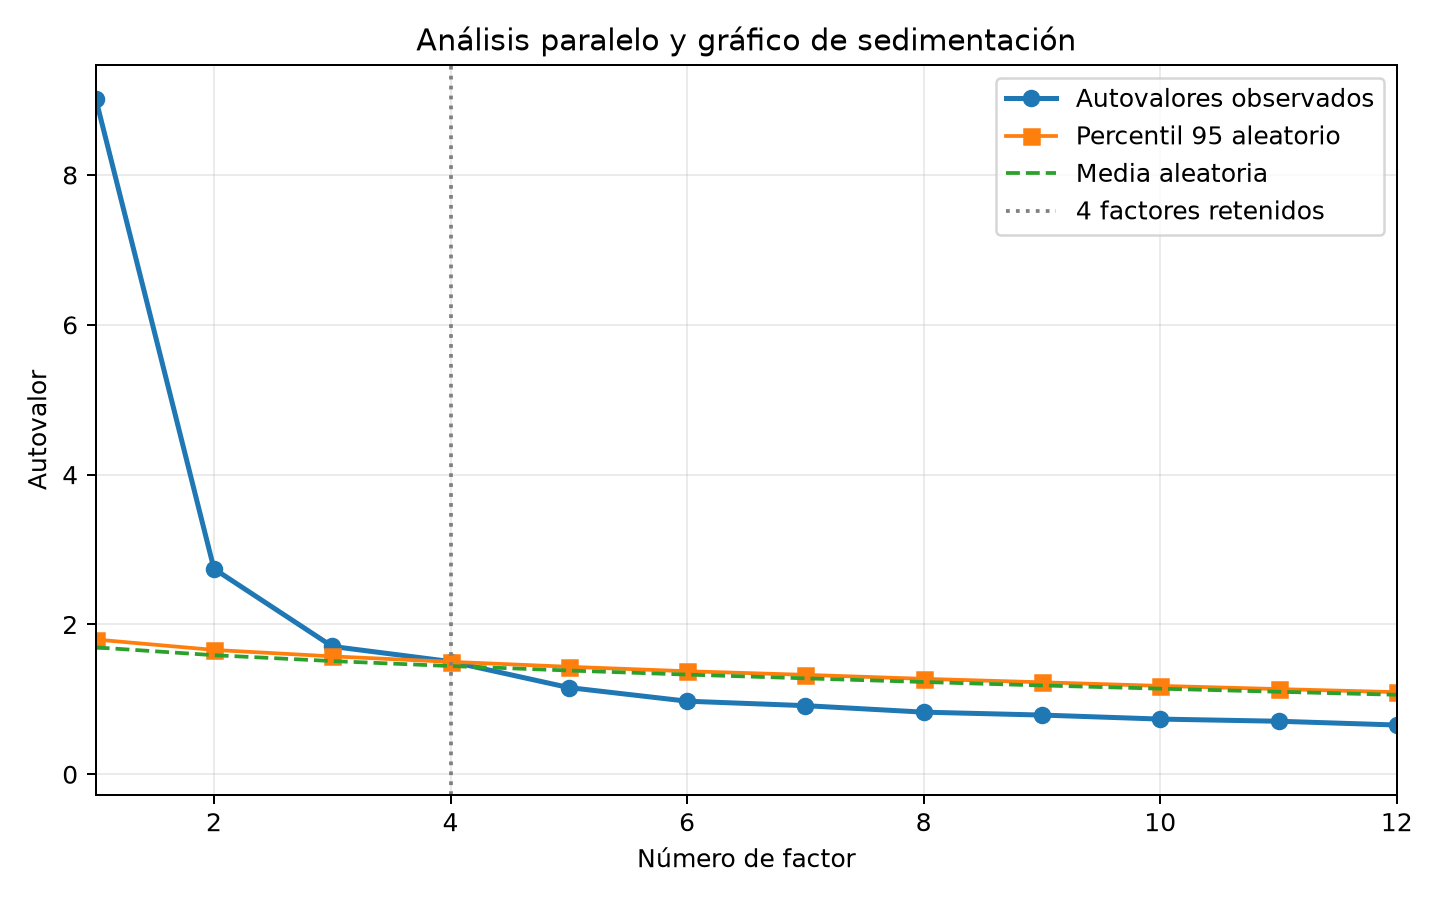
\includegraphics[width=0.78\textwidth]{assets/p2_scree_parallel.png}
\caption{Gráfico de sedimentación y análisis paralelo del EECS-R}
\end{figure}

\subsection*{Matriz patrón e interpretación}

La Tabla \ref{tab:patron} presenta las cargas de máxima verosimilitud con rotación Oblimin. Se considera sustantiva una carga absoluta cercana o superior a 0.40. Los cuatro factores explican en conjunto el 39.1\% de la varianza. El aporte por factor fue: F1=15.4\%, F2=9.7\%, F3=7.6\% y F4=6.3\%. Esta varianza acumulada es modesta, pero razonable en escalas actitudinales con ítems psicológicos y contenido heterogéneo; por eso la conclusión se formula como apoyo parcial y no como confirmación perfecta de la teoría.

\begin{table}[p]\centering
\caption{Matriz patrón rotada del EECS-R}
\label{tab:patron}
\small
\begin{tabular}{lrrrrl}
\toprule
Ítem & F1 & F2 & F3 & F4 & Interpretación dominante\\
\midrule
q1 & .40 & $-$.14 & .28 & .34 & Complejo\\
q2 & .10 & $-$.33 & .36 & .27 & Interpersonal débil\\
q3 & .12 & .29 & $-$.05 & .51 & Estadística\\
q4 & .12 & .17 & .14 & .51 & Estadística\\
q5 & .06 & .05 & .67 & $-$.13 & Interpersonal\\
q6 & .16 & $-$.35 & .16 & .26 & Interpersonal débil\\
q7 & .14 & .45 & $-$.05 & .30 & Enseñanza\\
q8 & .58 & .22 & .04 & .24 & Diseño experimental\\
q9 & .44 & $-$.11 & .26 & .37 & Complejo\\
q10 & .42 & $-$.07 & .18 & .04 & Diseño/enseñanza\\
q11 & .27 & .46 & .20 & .10 & Enseñanza\\
q12 & $-$.01 & .13 & .27 & $-$.16 & Débil\\
q13 & .56 & .08 & $-$.03 & .21 & Diseño experimental\\
q14 & .76 & .03 & .18 & $-$.34 & Diseño experimental\\
q15 & .36 & $-$.02 & .14 & .18 & Débil\\
q16 & .74 & .22 & $-$.02 & $-$.20 & Diseño experimental\\
q17 & .79 & $-$.01 & $-$.03 & .14 & Diseño experimental\\
q18 & .23 & $-$.32 & .40 & .14 & Interpersonal\\
q19 & $-$.05 & .57 & $-$.18 & .08 & Enseñanza\\
q20 & .04 & .45 & .05 & .20 & Enseñanza\\
q21 & .47 & .17 & $-$.04 & .27 & Diseño/estadística\\
q22 & .86 & $-$.07 & $-$.02 & .11 & Diseño experimental\\
q23 & $-$.09 & .04 & .70 & .07 & Interpersonal\\
q24 & .10 & .28 & .13 & .48 & Estadística\\
q25 & .10 & .53 & .13 & .08 & Enseñanza\\
q26 & .28 & .59 & .02 & $-$.07 & Enseñanza\\
q27 & $-$.02 & .61 & .38 & .07 & Complejo\\
q28 & .01 & .21 & .53 & $-$.02 & Interpersonal\\
\bottomrule
\end{tabular}
\end{table}

El primer factor representa principalmente entusiasmo por el diseño experimental; el segundo, amor por la enseñanza; el tercero, deficiencia de habilidades interpersonales; y el cuarto, amor por la estadística. Algunos ítems presentan complejidad porque sus enunciados combinan contenido estadístico, experimental y docente.

Una carga factorial puede interpretarse aproximadamente como la relación entre el ítem y el factor, controlando la estructura rotada. El signo indica dirección y la magnitud indica fuerza. Por ejemplo, q22 carga 0.86 en F1, por lo que es un indicador especialmente claro de entusiasmo por diseñar experimentos. En cambio, q12 no alcanza 0.40 en ningún factor, por lo que aporta poca información a una dimensión específica. Esto lo convierte en candidato a revisión o eliminación, porque no parece representar con claridad ninguna dimensión latente. Una carga cruzada ocurre cuando un ítem se relaciona materialmente con más de un factor; esto dificulta su interpretación y reduce la pureza de la escala.

Se eligió Oblimin porque una rotación ortogonal forzaría correlaciones iguales a cero entre amor por estadísticas, diseño y enseñanza, una restricción contraria al enunciado. Las correlaciones factoriales estimadas alcanzan 0.47 entre F1 y F3, lo que confirma que la restricción ortogonal habría sido inadecuada. La rotación no cambia la solución fundamental ni la varianza común total; facilita obtener una estructura psicológicamente interpretable.

La confiabilidad fue alta para diseño experimental ($\alpha=0.880$) y estadística ($\alpha=0.830$), adecuada para enseñanza ($\alpha=0.747$) y más baja para la dimensión interpersonal ($\alpha=0.691$), debido a ítems débiles y cruzados. Todas las correlaciones ítem--total dentro de cada conjunto son positivas, por lo que la menor consistencia interpersonal refleja heterogeneidad de contenido y no ítems invertidos. El alfa evalúa consistencia interna, no unidimensionalidad: un alfa alto significa que los ítems covarían, pero no sustituye el análisis de cargas. Por ello la evaluación conjunta considera cantidad de factores, contenido, cargas principales, cargas cruzadas y confiabilidad.


\subsection*{Ítems problemáticos y evaluación de la teoría}

La solución de cuatro factores es coherente con la teoría de Blend, pero no todos los ítems presentan una asignación limpia. La Tabla \ref{tab:p2_items_problematicos} resume los principales casos que deberían revisarse antes de validar una versión definitiva de la escala.

\begin{table}[H]\centering
\caption{Ítems problemáticos del EECS-R}
\label{tab:p2_items_problematicos}
\small
\begin{tabular}{p{1.6cm}p{6.5cm}p{5.0cm}}
\toprule
Ítem & Problema principal & Acción sugerida\\
\midrule
q1 & Carga cruzada entre factores & Revisar redacción\\
q9 & Carga cruzada entre diseño y estadística & Revisar redacción\\
q12 & No alcanza carga sustantiva en ningún factor & Eliminar o reformular\\
q15 & Carga débil & Revisar pertinencia\\
q27 & Carga cruzada entre enseñanza e interpersonal & Revisar redacción\\
q2 y q6 & Asociación débil con el factor interpersonal & Revisar contenido\\
\bottomrule
\end{tabular}
\end{table}

\begin{table}[H]\centering
\caption{Evaluación de la teoría de Blend}
\label{tab:p2_blend}
\small
\begin{tabular}{p{5.5cm}p{5.5cm}p{3.0cm}}
\toprule
Criterio & Resultado & Evaluación\\
\midrule
Número de factores esperados & El análisis paralelo retiene cuatro factores & Se cumple\\
Factores interpretables & Los factores son coherentes con diseño experimental, enseñanza, interpersonal y estadística & Se cumple\\
Correlación entre factores & La rotación oblicua es conceptualmente apropiada & Se cumple\\
Cargas factoriales limpias & Existen ítems débiles y con cargas cruzadas & Se cumple parcialmente\\
Confiabilidad & Adecuada en general, aunque más débil en la dimensión interpersonal & Se cumple parcialmente\\
\bottomrule
\end{tabular}
\end{table}

\subsection*{Conclusión de la pregunta 2}

La evidencia apoya parcialmente la teoría de Blend. En síntesis, el apoyo es estructuralmente fuerte, pero psicométricamente parcial. El análisis paralelo identifica cuatro factores, exactamente la cantidad propuesta por la teoría. Además, los factores obtenidos son interpretables y presentan una correspondencia razonable con las dimensiones teóricas de estadística, diseño experimental, enseñanza y habilidades interpersonales.

Sin embargo, el apoyo no es completo a nivel de ítems. Algunos reactivos presentan cargas cruzadas o cargas débiles, especialmente en la dimensión interpersonal. Por esta razón, la teoría recibe apoyo empírico general, pero la estructura observada no constituye una confirmación perfecta del cuestionario EECS-R.

Se recomienda revisar los ítems problemáticos y posteriormente validar una versión refinada mediante análisis factorial confirmatorio.

\section*{Pregunta 3}


\subsection*{Enunciado}

Como recién llegado a la consultora antes mencionada, le han incluido en un segundo proyecto, relacionado con los efectos de las condiciones de trabajo sobre la satisfacción y permanencia de los trabajadores. En este contexto, se han considerado los siguientes constructos relevantes para la investigación:

\begin{itemize}\itemsep2pt
\item \textbf{Actitud hacia compañeros de trabajo:} Actitud del empleado hacia/con sus compañeros de trabajo con los que interactúa regularmente.
\item \textbf{Percepción del ambiente de trabajo:} Percepción del trabajador respecto a su lugar de trabajo.
\item \textbf{Satisfacción con el trabajo:} Medición del nivel de satisfacción del empleado con su trabajo.
\item \textbf{Compromiso organizacional:} Grado en que el empleado se identifica y siente parte de la empresa.
\item \textbf{Intención de permanecer en el trabajo:} Grado en el que el trabajador pretende continuar trabajando para la empresa.
\item \textbf{Características personales:} Edad, Género, y experiencia en años del trabajador.
\end{itemize}

Cada uno de estos constructos fue medido en escalas de múltiples ítems que se describen a continuación, y que fueron aplicadas en un cuestionario a 400 empleados de diversas empresas del sector de telecomunicaciones (disponibles en el archivo \textit{Laboral.sav}):

\begin{figure}[H]
\centering
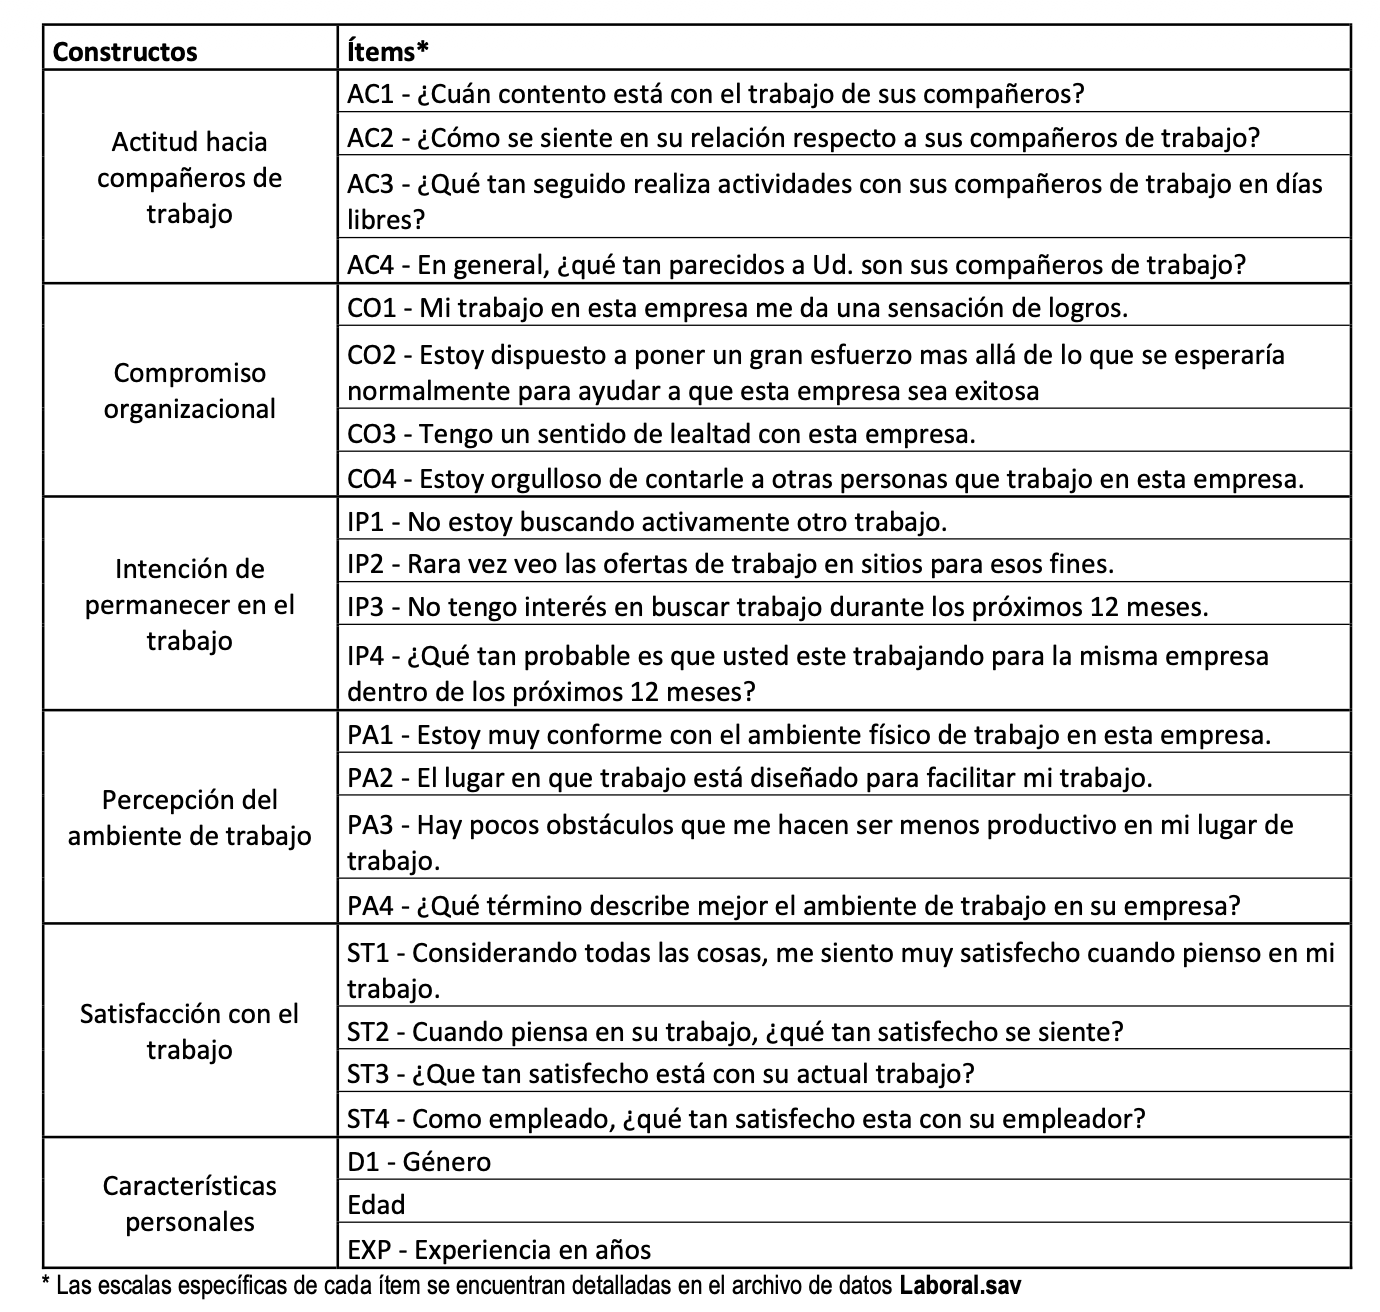
\includegraphics[width=0.95\textwidth]{assets/p3_tabla_constructos.png}
\caption{Constructos e ítems}
\end{figure}

Gracias a sus conocimientos en el área de comportamiento organizacional, usted ha identificado dos posibles modelos que expliquen la relación entre las condiciones de trabajo percibidas por el trabajador, y su satisfacción e intenciones de permanecer en la empresa. Estos modelos difieren principalmente en si el efecto de la precepción de ambiente de trabajo y la actitud hacia los compañeros de trabajo tienen efectos completamente mediados o parcialmente mediados sobre la intención de permanecer en la empresa.

Cada uno de los modelos se describe a continuación:

\begin{figure}[H]
\centering
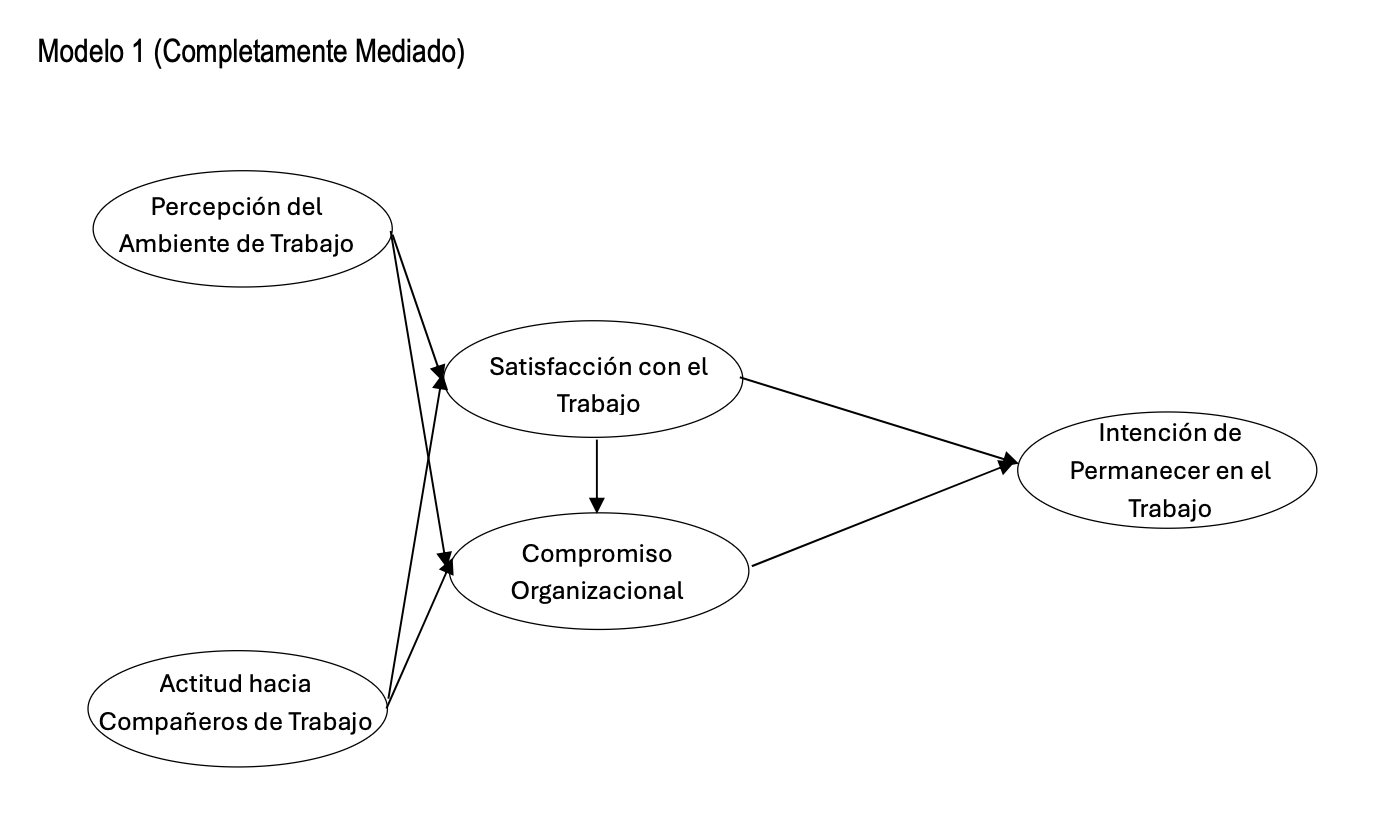
\includegraphics[width=0.78\textwidth]{assets/p3_modelo_completamente_mediado.png}
\caption{Modelo 1 (Completamente Mediado)}
\end{figure}

\begin{figure}[H]
\centering
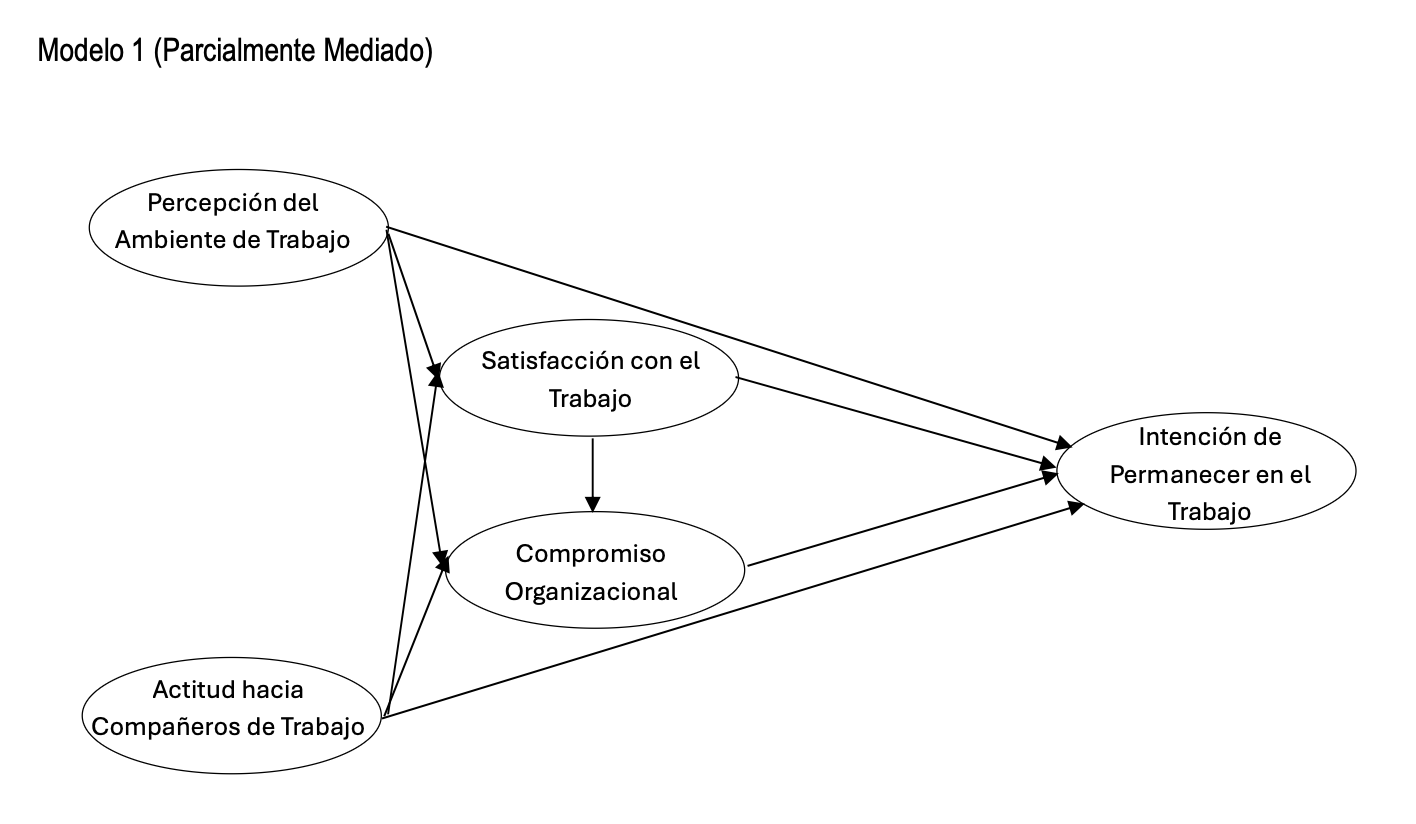
\includegraphics[width=0.78\textwidth]{assets/p3_modelo_parcialmente_mediado.png}
\caption{Modelo 1 (Parcialmente Mediado)}
\end{figure}

Su labor consiste en determinar:
\begin{enumerate}[label=\alph*)]\itemsep2pt
\item Qué tan bueno es el modelo de medición (incluyendo medidas de confiabilidad y validez de escalas).
\item Determinar cuál de los dos modelos representa de mejor forma los datos recopilados.
\item Para el modelo identificado como superior, evalúe si las relaciones entre las distintas variables se comportan de la misma forma entre hombres y mujeres.
\item Explique sus resultados y conclusiones.
\end{enumerate}

\subsection*{Respuesta}

\subsection*{Por qué corresponde CFA y SEM}

Los conceptos analizados no se observan directamente, sino mediante escalas compuestas por varios ítems. Por esta razón, primero se requiere evaluar si los indicadores representan adecuadamente sus constructos teóricos. Para ello se utiliza análisis factorial confirmatorio (CFA).

Una vez evaluado el modelo de medición, se utiliza modelamiento de ecuaciones estructurales (SEM) para comparar los dos modelos teóricos propuestos. Esta estrategia permite estimar simultáneamente las relaciones entre variables latentes, considerando el error de medición de los indicadores.

\subsection*{a) Evaluación del modelo de medición}

La base contiene 400 empleados y cinco constructos reflectivos, cada uno medido por cuatro indicadores: actitud hacia compañeros (AC), percepción del ambiente (PA), satisfacción laboral (ST), compromiso organizacional (CO) e intención de permanecer (IP).

\paragraph{Ajuste del CFA.} Se estimó primero un análisis factorial confirmatorio puro con los cinco constructos libremente correlacionados, sin restricciones estructurales. El ajuste fue muy bueno:
\[
\chi^2(160)=220.31,\quad \text{CFI}=0.985,\quad \text{TLI}=0.982,\quad \text{RMSEA}=0.031,
\]
superando con holgura los criterios usuales (CFI/TLI $\geq 0.95$; RMSEA $\leq 0.06$). La Tabla \ref{tab:cargas-cfa} reporta las cargas factoriales estandarizadas por ítem, que permiten evaluar cuantitativamente si cada indicador representa adecuadamente su constructo. Sobre estas cargas se calcularon la confiabilidad compuesta y la varianza media extraída:
\begin{equation}
CR=\frac{\left(\sum_i \lambda_i\right)^2}{\left(\sum_i \lambda_i\right)^2+\sum_i \theta_i},\qquad
AVE=\frac{\sum_i \lambda_i^2}{\sum_i \lambda_i^2+\sum_i \theta_i},
\end{equation}
donde $\lambda_i$ son las cargas estandarizadas y $\theta_i=1-\lambda_i^2$ los errores. CR resume la consistencia de los indicadores ponderando sus cargas y AVE indica cuánta varianza de los ítems captura el constructo frente al error.


\begin{table}[htbp]\centering
\caption{Cargas factoriales estandarizadas del CFA por ítem}
\label{tab:cargas-cfa}
\scriptsize
\begin{tabular}{llrrrr}
\toprule
Constructo & Ítem & Carga no est. & Carga est. & EE & $z$\\
\midrule
AC & AC1 & 1.000 & .822 & -- & --\\
AC & AC2 & 1.236 & .820 & .067 & 18.389\\
AC & AC3 & 1.038 & .837 & .055 & 18.867\\
AC & AC4 & 1.147 & .816 & .063 & 18.251\\
PA & PA1 & 1.000 & .692 & -- & --\\
PA & PA2 & 1.034 & .804 & .073 & 14.089\\
PA & PA3 & .820 & .778 & .060 & 13.727\\
PA & PA4 & .914 & .823 & .064 & 14.335\\
ST & ST1 & 1.000 & .737 & -- & --\\
ST & ST2 & 1.023 & .737 & .081 & 12.611\\
ST & ST3 & .929 & .697 & .077 & 12.092\\
ST & ST4 & .920 & .709 & .075 & 12.257\\
CO & CO1 & 1.000 & .584 & -- & --\\
CO & CO2 & 1.313 & .885 & .107 & 12.215\\
CO & CO3 & .782 & .657 & .076 & 10.327\\
CO & CO4 & 1.164 & .836 & .097 & 11.975\\
IP & IP1 & 1.000 & .811 & -- & --\\
IP & IP2 & 1.073 & .864 & .055 & 19.556\\
IP & IP3 & 1.066 & .741 & .066 & 16.053\\
IP & IP4 & 1.167 & .852 & .061 & 19.222\\
\bottomrule
\end{tabular}
\end{table}

\begin{table}[htbp]\centering
\caption{Calidad del modelo de medición (CFA)}
\begin{tabular}{lrrrrrr}
\toprule
Constructo & Alfa & CR & AVE & $\sqrt{AVE}$ & Carga mín. & Carga máx.\\
\midrule
AC & .891 & .894 & .679 & .824 & .815 & .837\\
PA & .847 & .858 & .602 & .776 & .692 & .823\\
ST & .811 & .811 & .518 & .720 & .697 & .737\\
CO & .823 & .834 & .564 & .751 & .584 & .885\\
IP & .886 & .890 & .670 & .818 & .741 & .864\\
\bottomrule
\end{tabular}
\end{table}

Las cargas estandarizadas oscilan entre .584 y .885; la mayoría supera .70 y las cargas inferiores pertenecen a escalas que mantienen CR y AVE adecuados. Todos los alfas y CR superan 0.70, y todas las AVE superan 0.50: existe confiabilidad y validez convergente adecuadas. Estos indicadores responden preguntas diferentes: alfa mide consistencia interna bajo supuestos relativamente restrictivos de equivalencia entre ítems; CR se basa en las cargas estimadas y es más apropiada dentro de CFA; AVE es la proporción promedio de varianza del indicador explicada por el constructo, de modo que AVE $>0.50$ significa que el constructo explica más varianza que el error.

\paragraph{Validez discriminante.} La correlación latente más alta implicada por el CFA es 0.562 (PA con IP), inferior a la menor raíz de AVE (0.720 en ST), por lo que se cumple el criterio de Fornell--Larcker: cada constructo comparte más varianza con sus indicadores que con los demás constructos. El HTMT máximo fue 0.569 (PA--IP), muy por debajo del umbral de 0.85. Existe validez discriminante: cada escala captura algo distinto.

La carga más baja fue 0.584 en CO1, todavía aceptable. No fue necesario eliminar ítems, evitando modificar el instrumento únicamente para mejorar el ajuste.

\paragraph{Conclusión del inciso a).} El modelo de medición es adecuado. Cuantitativamente, el CFA presenta buen ajuste global (CFI=0.985, TLI=0.982, RMSEA=0.031), todas las escalas tienen confiabilidad suficiente (alfas entre 0.811 y 0.891; CR entre 0.811 y 0.894), todos los AVE son superiores a 0.50 y el HTMT máximo es 0.569, inferior al umbral de 0.85. Por lo tanto, las escalas muestran confiabilidad, validez convergente y validez discriminante suficientes para continuar con la comparación de los modelos estructurales.

\subsection*{b) Selección del modelo estructural superior}

Se compararon dos modelos anidados según las flechas de las figuras del enunciado. El modelo completamente mediado permite que $PA$ y $AC$ expliquen $ST$ y $CO$, que $ST$ explique $CO$ e $IP$, y que $CO$ explique $IP$. El modelo parcialmente mediado mantiene esos caminos y agrega dos efectos directos adicionales: $PA\rightarrow IP$ y $AC\rightarrow IP$. Por tanto, el modelo completo se obtiene fijando en cero esos dos caminos directos, y la diferencia de $\chi^2$ prueba si liberarlos mejora el ajuste más de lo esperable por azar.

Los criterios de información se calcularon sobre el estadístico de ajuste, $AIC=\chi^2+2k$ y $BIC=\chi^2+k\ln n$, con $k$ el número de parámetros libres y $n=400$. Estas versiones son comparables entre modelos anidados estimados sobre los mismos datos; se prefieren valores menores.\footnote{No se utilizó el AIC/BIC que reporta \texttt{semopy} por defecto, porque se basa en el valor de la función de ajuste y no es comparable con el AIC clásico que reportan lavaan o AMOS.}

\begin{table}[htbp]\centering
\caption{Índices de ajuste estructural}
\begin{tabular}{lrrrrrrrr}
\toprule
Modelo & $\chi^2$ & gl & CFI & TLI & RMSEA & $k$ & AIC & BIC\\
\midrule
Completo & 267.13 & 162 & .974 & .969 & .040 & 48 & 363.13 & 554.72\\
Parcial & 220.31 & 160 & .985 & .982 & .031 & 50 & 320.31 & 519.88\\
\bottomrule
\end{tabular}
\end{table}

El modelo parcial presenta mejor CFI, TLI y RMSEA, y la prueba de diferencia entre modelos anidados es claramente significativa. La hipótesis nula de esta comparación es que los caminos directos agregados no mejoran el modelo; por tanto, si $p<0.05$ se rechaza esa restricción y se prefiere el modelo más flexible:
\[
\Delta\chi^2(2)=46.83,\quad p<0.001.
\]
AIC y BIC también favorecen al modelo parcial (diferencias de 42.83 y 34.84 puntos, respectivamente): la mejora de ajuste supera con creces la penalización por los dos parámetros adicionales. Considerando ajuste, significancia, criterios de información y contenido teórico, se seleccionó el \textbf{modelo parcialmente mediado}.

El $\chi^2$ evalúa ajuste exacto y suele ser sensible al tamaño muestral. CFI y TLI comparan el modelo con uno de independencia; valores cercanos o superiores a 0.95 representan buen ajuste. RMSEA estima error de aproximación por grado de libertad; 0.031 es compatible con muy buen ajuste. AIC y BIC penalizan complejidad, siendo BIC más severo; en este caso todos los criterios coinciden.

\paragraph{Relaciones estructurales del modelo seleccionado.}

\begin{table}[htbp]\centering
\caption{Coeficientes del modelo parcialmente mediado}
\begin{tabular}{lrrr}
\toprule
Relación & $B$ & $\beta$ estandarizado & $p$\\
\midrule
$PA\rightarrow ST$ & .1848 & .237 & $<.001$\\
$AC\rightarrow ST$ & $-$.0306 & $-$.036 & .554\\
$PA\rightarrow CO$ & .4969 & .427 & $<.001$\\
$AC\rightarrow CO$ & .2505 & .195 & $<.001$\\
$ST\rightarrow CO$ & .1306 & .087 & .110\\
$PA\rightarrow IP$ & .1975 & .354 & $<.001$\\
$AC\rightarrow IP$ & .0709 & .115 & .018\\
$ST\rightarrow IP$ & .0485 & .068 & .169\\
$CO\rightarrow IP$ & .1576 & .329 & $<.001$\\
\bottomrule
\end{tabular}
\end{table}

La percepción del ambiente incrementa la satisfacción, el compromiso y la intención de permanecer. La actitud hacia compañeros no predice satisfacción, pero sí compromiso y tiene un efecto directo pequeño sobre permanencia. Los coeficientes estandarizados muestran que el camino más fuerte es $PA\rightarrow CO$ ($\beta=.427$), seguido por $PA\rightarrow IP$ ($\beta=.354$) y $CO\rightarrow IP$ ($\beta=.329$). En cambio, $ST\rightarrow CO$ y $ST\rightarrow IP$ no son significativos al 5\% una vez incorporados los caminos directos desde $PA$ y $AC$.


\subsection*{c) Comparación de relaciones entre hombres y mujeres}

Se estimó el modelo parcialmente mediado por separado para hombres y mujeres. El ajuste fue adecuado en ambos grupos: hombres ($n=200$, CFI=.981, RMSEA=.031) y mujeres ($n=200$, CFI=.972, RMSEA=.041). Esto permite una comparación preliminar de los caminos estructurales entre grupos.

Cada coeficiente no estandarizado se comparó mediante:

\[
z = \dfrac{b_H-b_M}{\sqrt{SE_H^2+SE_M^2}}.
\]

\begin{table}[H]
\centering
\caption{Diferencias de relaciones estructurales por género}
\begin{tabular}{lcccc}
\toprule
Relación & Hombres & Mujeres & $z$ & $p$ \\
\midrule
$PA \rightarrow ST$ & .2594 & .1443 & 1.059 & .290 \\
$AC \rightarrow ST$ & -.2145 & .3509 & -3.313 & .001 \\
$PA \rightarrow CO$ & .6348 & .5099 & .743 & .457 \\
$AC \rightarrow CO$ & .3620 & 1.0379 & -2.418 & .016 \\
$ST \rightarrow CO$ & .0729 & .0830 & -.059 & .953 \\
$PA \rightarrow IP$ & .0984 & .2385 & -1.967 & .049 \\
$AC \rightarrow IP$ & -.0045 & .0038 & -.072 & .942 \\
$ST \rightarrow IP$ & .0601 & .0171 & .576 & .565 \\
$CO \rightarrow IP$ & .1327 & .2050 & -1.152 & .250 \\
\bottomrule
\end{tabular}
\end{table}

Los resultados muestran evidencia preliminar de diferencias entre hombres y mujeres en tres relaciones: $AC \rightarrow ST$, $AC \rightarrow CO$ y $PA \rightarrow IP$.

La diferencia más marcada aparece en $AC \rightarrow ST$. Entre hombres, la actitud hacia compañeros se relaciona negativamente con satisfacción laboral ($b=-.2145$), mientras que entre mujeres la relación es positiva ($b=.3509$). La diferencia entre ambos coeficientes es estadísticamente significativa ($z=-3.313$, $p=.001$). Este resultado debe interpretarse con cautela, ya que implica un cambio de signo entre grupos.

En $AC \rightarrow CO$, ambos efectos son positivos, pero el efecto es mayor entre mujeres ($b=1.0379$) que entre hombres ($b=.3620$), con una diferencia significativa ($z=-2.418$, $p=.016$). Esto sugiere que la actitud hacia los compañeros parece tener mayor importancia para explicar el compromiso organizacional en mujeres.

Finalmente, en $PA \rightarrow IP$, el efecto de la percepción del ambiente sobre la intención de permanecer también es mayor entre mujeres ($b=.2385$) que entre hombres ($b=.0984$), con una diferencia marginalmente significativa ($z=-1.967$, $p=.049$).

No se concluyen diferencias en las demás relaciones estructurales. Es importante destacar que no basta con observar que un coeficiente sea significativo en un grupo y no en otro; la comparación relevante es la diferencia directa entre coeficientes mediante el estadístico $z$.

La conclusión multigrupo debe interpretarse con cautela. En este trabajo se verifica ajuste adecuado por grupo y se comparan caminos estructurales, pero una comparación completa entre hombres y mujeres requeriría evaluar formalmente invariancia de medición, especialmente invariancia métrica.

\subsection*{d) Explicación y conclusión de los resultados}

El modelo de medición es sólido. El CFA presenta muy buen ajuste global y las escalas muestran confiabilidad, validez convergente y validez discriminante adecuadas. Por tanto, los constructos pueden utilizarse para evaluar las relaciones estructurales propuestas.

La comparación entre modelos muestra que el modelo parcialmente mediado representa mejor los datos que el modelo completamente mediado. Esto significa que las condiciones laborales no influyen sobre la intención de permanecer únicamente a través de satisfacción y compromiso, sino que también existen efectos directos desde la percepción del ambiente y la actitud hacia compañeros.

La percepción del ambiente de trabajo emerge como el antecedente más relevante del modelo. Se relaciona positivamente con satisfacción laboral, compromiso organizacional e intención de permanecer. Además, el compromiso organizacional constituye uno de los predictores más importantes de la permanencia laboral.

En cambio, la satisfacción laboral no presenta efectos significativos sobre compromiso ni sobre intención de permanecer una vez incorporadas las demás relaciones del modelo. Esto sugiere que, en esta muestra, la permanencia laboral depende más directamente de la percepción del ambiente y del compromiso organizacional que de la satisfacción laboral por sí sola.

Respecto de la comparación por género, se observa evidencia preliminar de diferencias en tres caminos estructurales: $AC \rightarrow ST$, $AC \rightarrow CO$ y $PA \rightarrow IP$. Estas diferencias sugieren que algunas relaciones laborales podrían operar con distinta intensidad entre hombres y mujeres. Sin embargo, esta conclusión debe considerarse exploratoria, porque no se realizó una prueba formal de invariancia métrica del modelo de medición.

En conjunto, la evidencia respalda el modelo parcialmente mediado como la representación más adecuada de las relaciones entre ambiente laboral, satisfacción, compromiso e intención de permanecer en la organización.

\section*{Pregunta 4}


\subsection*{Enunciado}

La empresa HBAT produce y vende productos de papel a dos industrias: Impresores de revistas e impresores de diarios. Los productos llegan a estos clientes a través de dos canales: Directo (Fuerza de Ventas) e Indirecto (Agentes). HBAT realizó una investigación de mercados en las que recolectó información en un sinnúmero de variables (métricas y no métricas, disponibles en el archivo \textit{HBAT200.sav}) en una muestra de 200 clientes.

Entre las variables consideradas se encuentran algunas asociadas al resultado de compras y relación (5 variables), y variables descriptivas de las empresas de las cuales se recolecto información. Las variables se describen a continuación:

\textbf{Datos de Clasificación de las empresas encuestadas}
\begin{itemize}\itemsep2pt
\item X1 - Tipo de Cliente.
\item X2 - Tipo de Industria.
\item X3 - Tamaño de la Empresa.
\item X4 - Región.
\item X5 - Sistema de Distribución.
\end{itemize}

\textbf{Resultado de Compras y Relación con HBAT}
\begin{itemize}\itemsep2pt
\item X19 - Satisfacción.
\item X20 - Intención de Recomendar a HBAT.
\item X21 - Intención de Recomprar a HBAT.
\item X22 - Nivel de Compras de HBAT.
\item X23 - Considera Alianza Estratégica con HBAT.
\end{itemize}

Los ejecutivos de HBAT tienen diversas preguntas respecto a su desempeño y el nivel de satisfacción de sus clientes. En particular, están interesados en conocer el efecto de ``Tamaño de la Empresa'' y el ``Tipo de Distribución'' en la lealtad de los clientes, la cual consideran un constructo compuesto por tres variables (X19: Satisfacción, X20: Intención de Recomendar, X21: Intención de Recomprar). En particular, desean determinar si:

\begin{enumerate}[label=\alph*)]\itemsep2pt
\item \textquestiondown{}Incide el tipo de distribución en la lealtad de los clientes?
\item \textquestiondown{}Se comportan los clientes de forma distinta en términos de su lealtad dependiendo de su tamaño?
\item \textquestiondown{}Son las variables tipo de distribución y tamaño antecedentes independientes de la lealtad?
\end{enumerate}

\subsection*{Respuesta}

\subsection*{Por qué corresponde MANOVA}

La lealtad no se observa como una sola variable, sino como un perfil de tres respuestas relacionadas: satisfacción, recomendación y recompra. Por eso existen tres resultados que representan conjuntamente la lealtad. Ejecutar tres ANOVA independientes desde el inicio aumentaría el riesgo de error tipo I y perdería la información contenida en sus correlaciones. MANOVA contrasta primero si los grupos difieren en alguna combinación lineal de satisfacción, recomendación y recompra.

El diseño es factorial porque se analizan simultáneamente dos antecedentes categóricos. Esto permite separar dos efectos principales y una interacción. La interacción es indispensable para responder la tercera pregunta: si resulta significativa, el efecto de distribución depende del tamaño y los antecedentes no pueden describirse como independientes.

\subsection*{Diseño, procedimiento e hipótesis}

La lealtad se representa mediante satisfacción, intención de recomendar e intención de recomprar. Los antecedentes son tipo de distribución (indirecta con agente frente a directa) y tamaño de la empresa (pequeña frente a grande). Se aplicó MANOVA factorial $2\times2$ con celdas de 45, 63, 53 y 39 clientes.
\begin{align*}
H_{01}&:\ \text{el tipo de distribución no afecta conjuntamente la lealtad},\\
H_{02}&:\ \text{el tamaño no afecta conjuntamente la lealtad},\\
H_{03}&:\ \text{no existe interacción distribución}\times\text{tamaño}.
\end{align*}

La escala compuesta presenta alta consistencia ($\alpha=0.876$), con correlaciones entre indicadores de 0.66 a 0.76. Box M no fue significativo, $\chi^2(18)=27.55$, $p=0.069$, apoyando igualdad de matrices de covarianza. Levene fue significativo para satisfacción y recompra, pero no para recomendación; por ello se interpretaron conjuntamente las pruebas multivariadas y las medias, considerando la robustez derivada de tamaños de celda razonablemente balanceados. En un diseño $2\times2$ los efectos tienen un grado de libertad en el numerador, por lo que Pillai, Wilks, Hotelling y Roy producen exactamente el mismo $F$; se reporta Wilks por convención.

Además se requiere independencia entre clientes, ausencia de casos multivariados extremadamente influyentes, relaciones aproximadamente lineales entre resultados y ausencia de multicolinealidad perfecta. Box M contrasta igualdad de matrices de covarianza; no rechazarlo favorece el supuesto. Levene estudia igualdad de varianzas por resultado; sus resultados mixtos aconsejan cautela con los ANOVA, pero no invalidan la prueba multivariada.

\subsection*{Resultados MANOVA}

La lógica del contraste es comparar la variación dentro de los grupos con la variación atribuible a cada efecto. Wilks se expresa como razón de determinantes,
\[
\Lambda = \frac{|E|}{|E+H|},
\]
donde $E$ es la matriz de error y $H$ la matriz asociada al efecto. Un $\Lambda$ cercano a uno implica poca separación multivariada; un valor menor, acompañado de un $p$ significativo, indica que los vectores de medias difieren.

\begin{table}[htbp]\centering
\caption{Efectos multivariados sobre lealtad}
\begin{tabular}{lrrrrr}
\toprule
Efecto & Wilks $\Lambda$ & $F$ & gl$_1$ & gl$_2$ & $p$\\
\midrule
Distribución & .8526 & 11.184 & 3 & 194 & $<.001$\\
Tamaño & .9028 & 6.959 & 3 & 194 & $<.001$\\
Distribución$\times$Tamaño & .9034 & 6.917 & 3 & 194 & $<.001$\\
\bottomrule
\end{tabular}
\end{table}

Como $p<0.05$ en los tres contrastes, se rechazan las tres hipótesis nulas. Tanto distribución como tamaño influyen en la combinación de variables de lealtad y, además, interactúan: no son antecedentes independientes. Wilks $\Lambda$ representa la proporción de variación multivariada no explicada por el efecto. La interacción significativa es la evidencia formal de que la ventaja de un canal no es constante en ambos tamaños.

\subsection*{ANOVA univariados}

\begin{table}[htbp]\centering
\caption{Pruebas univariadas posteriores}
\begin{tabular}{llrrr}
\toprule
Resultado & Efecto & $F(1,196)$ & $p$ & $\eta_p^2$\\
\midrule
Satisfacción & Distribución & 118.934 & $<.001$ & .378\\
 & Tamaño & 27.977 & $<.001$ & .125\\
 & Interacción & 17.258 & $<.001$ & .081\\
\addlinespace
Recomendación & Distribución & 83.116 & $<.001$ & .298\\
 & Tamaño & 43.401 & $<.001$ & .181\\
 & Interacción & 1.506 & .221 & .008\\
\addlinespace
Recompra & Distribución & 55.402 & $<.001$ & .220\\
 & Tamaño & 29.988 & $<.001$ & .133\\
 & Interacción & 6.793 & .010 & .033\\
\bottomrule
\end{tabular}
\end{table}

Los ANOVA posteriores no sustituyen a MANOVA: explican qué resultados contribuyen al efecto conjunto, y se acompañan del tamaño de efecto $\eta_p^2=SC_{efecto}/(SC_{efecto}+SC_{error})$. La interacción se concentra en satisfacción ($\eta_p^2=.081$) y recompra ($\eta_p^2=.033$); para recomendación los efectos son esencialmente aditivos.

\subsection*{Medias e interpretación}

\begin{table}[htbp]\centering
\caption{Medias de lealtad por distribución y tamaño}
\begin{tabular}{llrrr}
\toprule
Distribución & Tamaño & Satisfacción & Recomendación & Recompra\\
\midrule
Indirecta & Pequeña & 6.211 & 6.091 & 7.142\\
Indirecta & Grande & 6.406 & 6.771 & 7.475\\
Directa & Pequeña & 7.128 & 7.079 & 7.670\\
Directa & Grande & 8.449 & 8.067 & 8.569\\
\bottomrule
\end{tabular}
\end{table}

Las medias permiten traducir la interacción. En satisfacción, la diferencia directa--indirecta es aproximadamente 0.92 puntos entre empresas pequeñas, pero 2.04 entre grandes. En recompra, la diferencia pasa de 0.53 a 1.09. Las líneas de medias, por tanto, no serían paralelas. Para recomendación las diferencias son 0.99 y 1.30, patrón más cercano al paralelismo y coherente con la interacción no significativa.

Los efectos simples se contrastaron con 12 pruebas $t$ de Welch. Con corrección de Bonferroni por familia ($\alpha=0.05/4=0.0125$ por variable dependiente) todas las conclusiones se mantienen: los contrastes significativos conservan $p<0.0125$ y los no significativos, como la diferencia grande--pequeña bajo distribución indirecta en satisfacción ($p=.347$) y recompra ($p=.064$), siguen siéndolo.

Los efectos principales deben interpretarse condicionados por la interacción: afirmar solamente que el canal directo es mejor ocultaría que su ventaja es especialmente marcada en empresas grandes. Por ello, la recomendación gerencial se basa en efectos simples y no únicamente en promedios marginales.

\subsection*{a) Incidencia del tipo de distribución}

El efecto multivariado del tipo de distribución es significativo: Wilks $\Lambda=.8526$, $F(3,194)=11.184$, $p<.001$. Se rechaza la hipótesis nula de igualdad. Los ANOVA muestran que el canal afecta satisfacción, recomendación y recompra, todos con $p<.001$, y las medias son sistemáticamente mayores bajo distribución directa. Por tanto, el tipo de distribución sí incide en la lealtad.

\subsection*{b) Diferencias de lealtad según tamaño}

El efecto multivariado del tamaño también es significativo: Wilks $\Lambda=.9028$, $F(3,194)=6.959$, $p<.001$. Los tres ANOVA univariados presentan diferencias significativas. Las empresas grandes muestran mayores niveles medios de satisfacción, recomendación y recompra. Por tanto, los clientes se comportan de forma distinta según el tamaño de su empresa.

\subsection*{c) Independencia entre distribución y tamaño}

La interacción distribución$\times$tamaño es significativa: Wilks $\Lambda=.9034$, $F(3,194)=6.917$, $p<.001$. Se rechaza la hipótesis de independencia. La ventaja del canal directo es mayor entre empresas grandes, especialmente en satisfacción y recompra. Por ello, distribución y tamaño no son antecedentes independientes de la lealtad.

\subsection*{Interpretación general de la pregunta 4}

El tipo de distribución y el tamaño inciden significativamente en la lealtad, pero no operan de manera independiente: el efecto favorable de la distribución directa se intensifica en empresas grandes, especialmente en satisfacción y recompra. Desde una perspectiva gerencial, HBAT debería priorizar el canal directo para clientes grandes, sin asumir que el mismo incremento de lealtad se producirá con igual magnitud en clientes pequeños.


\subsection*{Conclusión ejecutiva de la pregunta 4}

El tipo de distribución y el tamaño de la empresa influyen significativamente sobre la lealtad de los clientes. La distribución directa se asocia con mayores niveles de satisfacción, recomendación y recompra. Sin embargo, este efecto no es homogéneo para todos los clientes: la ventaja del canal directo es considerablemente mayor entre empresas grandes, particularmente en satisfacción y recompra.

Por tanto, distribución y tamaño no pueden considerarse antecedentes independientes de la lealtad. Desde una perspectiva gerencial, HBAT debería priorizar el canal directo especialmente para clientes de mayor tamaño.


\section*{Conclusión general}

Los cuatro análisis muestran que las relaciones estudiadas no pueden interpretarse como asociaciones simples entre variables aisladas. En la primera pregunta, la evidencia indica que la presión competitiva se transforma en desempeño innovador principalmente cuando activa la conducta innovadora de los empleados, y que este mecanismo es más fuerte en organizaciones con mayor tolerancia al fracaso.

En la segunda pregunta, el análisis factorial exploratorio entrega apoyo parcial a la teoría de Blend. La estructura de cuatro factores aparece en los datos y los factores son interpretables, pero algunos ítems presentan cargas cruzadas o débiles. Por ello, el cuestionario EECS-R requiere depuración antes de ser validado como instrumento definitivo.

En la tercera pregunta, el modelo de medición presenta evidencia adecuada de confiabilidad y validez, y el modelo parcialmente mediado representa mejor los datos que el modelo completamente mediado. La permanencia laboral depende especialmente de la percepción del ambiente de trabajo y del compromiso organizacional, aunque existe evidencia preliminar de que algunas relaciones podrían variar entre hombres y mujeres.

Finalmente, la cuarta pregunta muestra que la lealtad hacia HBAT depende tanto del canal de distribución como del tamaño del cliente, pero estos factores no operan de manera independiente. La distribución directa es especialmente favorable para empresas grandes, lo que sugiere que la estrategia comercial debería diferenciarse según el perfil del cliente.

En conjunto, la tarea ilustra la utilidad de técnicas multivariadas para responder preguntas distintas: mediación moderada para estudiar mecanismos condicionales, análisis factorial exploratorio para evaluar estructuras latentes emergentes, CFA/SEM para validar medición y comparar modelos causales teóricos, y MANOVA factorial para analizar perfiles de resultados relacionados entre grupos. Todos los cálculos pueden reproducirse en los cuatro notebooks individuales incluidos en la carpeta de entrega.

\end{document}
